%template1.tex
%The following LaTeX source file represents the simplest kind of slide presentation; no overlays, no included graphics. Substitute your favorite style for ``pascal''. To create the PDF file template1.pdf, (1) be sure to use the prosper class, then (2) execute the command latex template1.tex, and (3) the command dvipdf template1.dvi.

%%%%%%%%%%%%%%%%%%%%%%%%%%%%%%% template1.tex %%%%%%%%%%%%%%%%%%%%%%%%%%%%%%%%%%%
\documentclass[a4paper,blends,pdf,colorBG,slideColor]{prosper}
% definitions for slides for CSC544
% Lutz Hamel, (c) 2007

\hypersetup{pdfpagemode=FullScreen}

\usepackage{times}
\usepackage{latexsym}
\usepackage{alltt}
\usepackage{booktabs}
\usepackage{amsmath}
\usepackage{amsopn}
\usepackage{amsfonts}
\usepackage{amssymb}
%\usepackage[usenames]{color}

\def\sign{\qopname\relax{no}{sign}}
\def\argmax{\qopname\relax{no}{argmax}}
\def\argmin{\qopname\relax{no}{argmin}}

\newcommand{\grad}{\ensuremath{\nabla}} 
\newcommand{\loss}{\ensuremath{{\cal L}}}
\newcommand{\err}{\mbox{err}}
\newcommand{\mse}{\mbox{mse}}
\newcommand{\acc}{\mbox{acc}}
\newcommand{\Integer}{\ensuremath{\mathbb{N}}}
\newcommand{\size}[1]{{|{#1}|}}
\newcommand{\Rnspace}[1]{\ensuremath{\mathbb{R}^{#1}}}
\newcommand{\Real}{\ensuremath{\mathbb{R}}}
\newcommand{\mytt}[1]{{\small\tt{#1}}}
\newcommand{\textemph}[1]{{\em #1}}
\newcommand{\suchthat}{\mid}
\newcommand{\orbar}{\;|\;}
\newcommand{\bs}[1]{\begin{slide}{#1}\ptsize{8}}
\newcommand{\es}{\end{slide}}
\newcommand{\co}{\,\colon\;}
\newcommand{\pair}[2]{\ensuremath{( {#1}, {#2} )}}
\newcommand{\model}[1]{\hat{#1}}
\newcommand{\ul}[1]{{\bf\em #1}}
\newcommand{\ol}{\overline}
\newcommand{\definition}[1]{{\bf Definition: }{\em #1}}
\newcommand{\example}[1]{{\bf Example: }{#1}}
\newcommand{\abs}[1]{|{#1}|}
\newcommand{\mytab}{\makebox[.1in]{}}

\newcommand{\fdef}[1]{
\begin{center}
\fbox{
\begin{minipage}{3.5in}
{\bf Definition:}
{#1}
\end{minipage}
}
\end{center}
}

\newcommand{\fframe}[1]{
\begin{center}
\fbox{
\begin{minipage}{3.5in}
{#1}
\end{minipage}
}
\end{center}
}

\newcommand{\nframe}[1]{
\begin{center}
\begin{minipage}{3.5in}
{#1}
\end{minipage}
\end{center}
}

\newenvironment{Rcode}
	{
		\scriptsize
		\begin{quote}
		\begin{alltt}
	}
	{
		\end{alltt}
		\end{quote}
	}




\begin{document}

\bs{Statistical Learning Theory}
Up to this point we have developed support vector machines purely based on
\begin{itemize}
\item linear algebra 
\item maximum margin
\end{itemize}

$\Rightarrow$ The key insight was that the maximum margin
classifier is the best classifier when considering all possible hyperplanes
that separate two classes -- we based this argument on optimization theory.

Here we will look at 
{\em statistical learning
theory} that makes the notion of maximum margin classifier as the optimal classifier rigorous via statistical arguments.

At the heart of this theory is the notion of {\em VC-dimension}.

\es

\bs{VC-Dimension}
Informally, the VC-dimension is a 
measure of the {\em complexity of a classifier}.

It is a measure of how well the classifiers can separate the points
in the input space or model these points without any error.

\es

\bs{VC-Dimension}
More formally, consider the class of all classifiers with a margin
$\gamma$ of some fixed size, let $\hat{F}[\gamma]$ be that class.  

Now consider some dataset
$D$, then the {\em VC-dimension} of classifiers with the margin
$\gamma$ is the size of the largest subset of 
points from $D$ that can be separated
by classifiers in $\hat{F}[\gamma]$
without any errors for {\em all possible binary label assignments}.

If all points in $D$ can be separated for all possible
label assignments then we say that $\hat{F}[\gamma]$ {\em shatters} the dataset $D$.

\fdef{The {\em VC-dimension} of a model class $\hat{F}[\gamma]$ defined over some data set $D$ is the size of the largest finite subset of $D$ shattered by $\hat{F}[\gamma]$. 
}

\es

\bs{VC-Dimension}
\small
{\bf Example:} Consider a class of classifiers $\hat{F}[\gamma_1]$ with $\gamma_1$
denoting a margin of some fixed size.  

Let our dataset 
be a set of points in two dimensional real space, $D \subset \Rnspace{2}$.  

Let $\abs{D} = 3$, that is $D$ contains three points.

Given a size of $\gamma_1$ such that we can
separate all three points for all possible label assignments, then the VC-dimension is,
\[
h_1 = 3.
\]

\vspace{.1in}
\begin{center}
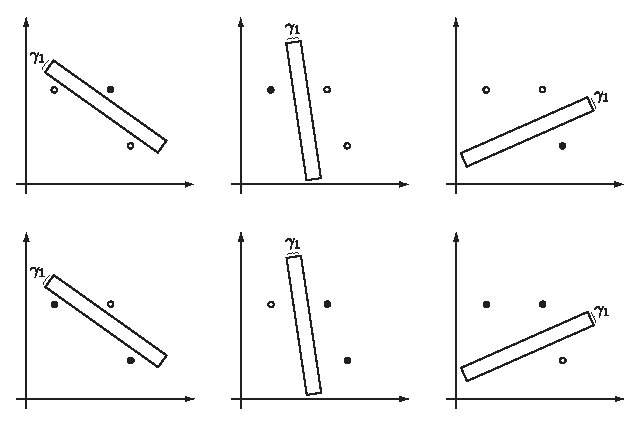
\includegraphics[height=35mm]{figures/fig10-02.eps}
\end{center}
Now, since $h = \abs{D}$, we say that $\hat{F}[\gamma_1]$ shatters $D$.
\es

\bs{VC-Dimension}
\small
{\bf Example:} Consider a second class of classifiers $\hat{F}[\gamma_2]$ over the same dataset $D$
with $\gamma_2 > \gamma_1$.  In particular, the size of $\gamma_2$ is such that
the classifiers will not be able to separate all points perfectly. 
\begin{center}
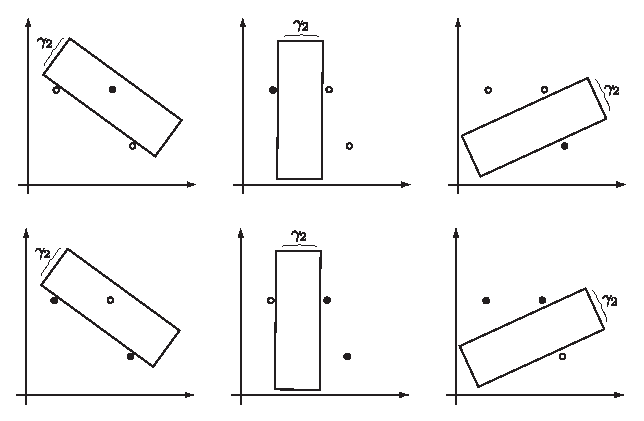
\includegraphics[height=35mm]{figures/fig10-03.eps}
\end{center}

Here we see that the maximum number of points that can be
separated by the classifiers in $\hat{F}[\gamma_2]$ is 2.  Therefore, we say that the
VC-dimension is $h_2 = 2$.

Observe that with $\gamma_2 > \gamma_1$ we have $h_2 < h_1$, that is, models with large
margins are less complex that models with small margins.
\es


\bs{VC-Dimension}

High VC-dimension numbers represent classes of models with high complexity and vice versa,
\[
\mbox{Model Complexity $\propto$ VC-Dimension}.
\]
The VC-dimension can be thought of as a formalization of the trade-off between
complexity and accuracy of a model.  
Classifiers with small margins and large VC-dimensions
will induce accurate but very
complex decision surfaces whereas classifiers with large
margins and small VC-dimensions will induce less accurate
and less complex decision surfaces.

It turns out that statistical learning theory sheds some light on exactly 
this trade-off in what is called {\em expected risk minimization}.
\es

\bs{VC-Dimension}

{\bf Observation:} The VC-dimension of a classifier is {\em data dependent}.
\begin{center}
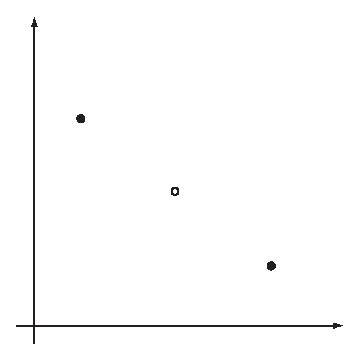
\includegraphics[height=35mm]{figures/fig10-05.eps}
\end{center}

Note, the above dataset VC-dimension $h=2$
regardless the size of the margin $\gamma$ in the class of classifiers $\hat{F}[\gamma]$
considered for modeling this dataset.
\es


\bs{Mathematical Expectation}
\[
E[g] = \int_x g(x) P(x) dx,
\]
where $g(x)$ is a function over some domain $X$ such that $x\in X$
and $P(x)$ is a probability distribution over $X$.

$E[g]$ represents the sum of function evaluations over the domain
$X$ weighted by their probabilities.  

If the domain $X$ is discrete with $k$ elements $x_1,\ldots,x_k$, then the expectation is expressed as,
\begin{equation*}
E[g] = \frac{1}{k} \sum_{i = 1}^{k} g(x_i).
\end{equation*}

Typically we call the expected value $E[f]$ the {\em average} or {\em mean} over 
all function evaluation over the domain $X$.

\es

\bs{Expected Risk}
Assume that $P(\ol{x},y)$ is the joint probability of the data instances
$\ol{x}\in \Rnspace{n}$ and their corresponding labels $y\in \{+1,-1\}$, 
also assume that $L$ is the 0-1 loss function,
then the \textemph{expected loss}
for some model $\model{f}\in \model{F}[\gamma]$ defined over the data universe is,
\begin{equation*}
E[L(y,\model{f}(\ol{x}))] = \int  L(y,\model{f}(\ol{x}))\: dP(\ol{x},y).
\end{equation*}
In other words, the expected loss is the expected number of mistakes a model will
commit over the underlying data universe.

We often write
\begin{equation*}
R[\model{f}] = E[L(y,\model{f}(\ol{x}))],
\end{equation*}
where $R[\model{f}]$ is called the \textemph{expected risk}.
\es

\bs{Risk Minimization}
The goal in statistical learning
is to find a model $\hat{f}^* \in \hat{F}$ that minimizes the
expected risk 
\[
\hat{f}^* = \argmin_{\hat{f} \in \hat{F}}R[\hat{f}],
\]
where $\model{F}$ represents the class of all model classes such
that $\model{F}[\gamma] \subset \model{F}$ for all margins $\gamma$.

Unfortunately, this is impossible in the
present formulation of the expected risk because we do not know the
probability distribution $P(\ol{x}, y)$.  

If we did, there would be nothing
to learn.  
\es

\bs{Empirical Risk}
\small
However, we do have some information on the joint probability distribution
in the form of samples in our dataset $D$,
\begin{equation*}
D = \{(\ol{x}_1,y_1),\ldots,(\ol{x}_l,y_l)\} \subset \Rnspace{n}\times \{+1,-1\}.
\end{equation*}

We can use these samples to
estimate the risk, we call this the {\em empirical risk} $R_{\text{emp}}[\model{f}]$ of some
model $f \in F$ and define
it as
\begin{equation*}
R_{\text{emp}}[\model{f}] = E[L(y, \model{f}(\ol{x}))] = \frac{1}{l}\sum_{i = 1}^l L(y_i, \model{f}(\ol{x}_i)),
\end{equation*}
where $(\ol{x}_i,y_i) \in D$.  Then,
\begin{align*}
\model{f}^* &= \argmin_{\model{f}\in\model{F}} R_{\text{emp}}[\model{f}] \\
\label{eq:min-empirical-risk}
	&= \argmin_{\model{f}\in\model{F}}  \left ( \frac{1}{l}\sum_{i = 1}^l L(y_i, \model{f}(\ol{x}_i)) \right ).
\end{align*}


However, minimizing this equation 
is overly optimistic, since we can always find some model which fits the
sample data extremely well.\footnote{Compare this to the training error of a model.}
\es

\bs{VC-Confidence}
\small
In order to use the empirical risk for
estimating the best model for the expected risk, Vapnik introduced a new term
called the {\em VC-confidence} which together with the empirical risk can be
considered a bound on the expected risk,
\[
R[\hat{f}] \leq \underbrace{R_{\text{emp}}[\hat{f}] + \overbrace{v(l,h,\eta)}^{\mbox{\small VC-confidence}}}_{\mbox{\small VC generalization bound}},
\]
where $h$ is the VC-dimension of $\hat{f}$ and $\eta$ is some small number such that
$0 < \eta < 1$. Typically $\eta = 0.05$ for the $95\%$ confidence interval, since
the theory states that the bound holds with probability
$1 - \eta$.

The VC-confidence term is defined as follows,
\[
v(l,h,\eta) = \sqrt{\frac{h(log(\frac{2l}{h})+1) - log(\frac{\eta}{4})}{l}}.
\]
Notice that the right side of the above equations 
do not depend the joint probability distribution $P(\ol{x},y)$.

{\bf Observation:} $v$ is directly proportional to $h$ and indirectly proportional to the number 
of training instances $l$.
\es

\bs{Generalization Bound}
\small
\begin{center}
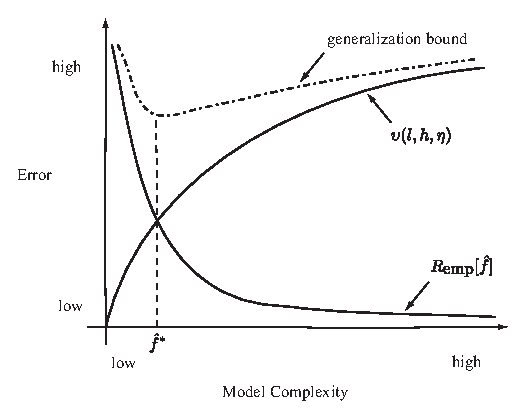
\includegraphics[height=35mm]{figures/fig10-06.eps}
\end{center}
The figure illustrates the relationship between
the empirical risk $R_{\text{emp}}[\hat{f}]$ and the VC-confidence $v(l,h,\eta)$.

Note that as the complexity of the models increases the empirical risk
decreases.  
That is, complex models allow us to model the training data well.

On the other hand, as model complexity increases so does the VC-confidence.  
Here, complex models will commit more errors on data not contained in the training data.

The generalization bound can be considered the envelope of these two curves.
It is interesting to note that minimizing the generalization bound
is equivalent to making just the right trade-off between model complexity
and error rate $\Rightarrow \hat{f}^*$.

\es

\bs{Structural Risk Minimization}
With the generalization bound we now have a way to characterize models that optimally trade off complexity and error.

The question remains,
how do we find these models?  

Our notion of model class $\hat{F}$ is most likely
infinite and we have to traverse this class of models to find the optimal
model $\hat{f}^*$ that minimizes the generalization bound. 

An effective way to traverse this model class in search for an optimal model
is {\em structural risk minimization}.
\es

\bs{Structural Risk Minimization}

suppose we have a class of linear models $\model{F}$ with 
\begin{equation*}
\model{F}[\gamma_1],\ldots,\model{F}[\gamma_k] \subset \model{F},
\end{equation*}
where
\begin{equation*}
\model{F}[\gamma_1] \subset \model{F}[\gamma_2] \subset \ldots \subset \model{F}[\gamma_k] \text{ if }
h_1 < h_2 < \ldots < h_k,
\end{equation*}
where $h_i$ is the VC-dimension of model class $\model{F}[\gamma_i]$.  

Given that we assume linear models, the equation above implies that the margins of the various model
classes are also partially ordered,
\begin{equation*}
\gamma_k <\ldots < \gamma_2 < \gamma_1. 
\end{equation*}
This gives us an effective procedure to find the optimal model:  We start with the least
complex model class $\model{F}[\gamma_1]$ and minimize the generalization bound.
We then move on to the next model class, in this case $\model{F}[\gamma_2]$,
and compute the optimal model $\model{f}_2^*$ in a similar fashion.
We terminate our search if we find that the generalization bound of some
model $\model{f}_{i+1}^*\in \model{F}[\gamma_{i+1}]$ is larger than the generalization
bound of the model $\model{f}_i^*\in \model{F}[\gamma_i]$.
In this case, $\model{f}_i^*$ is the optimal model.


\es

\bs{Structural Risk Minimization}
\begin{center}
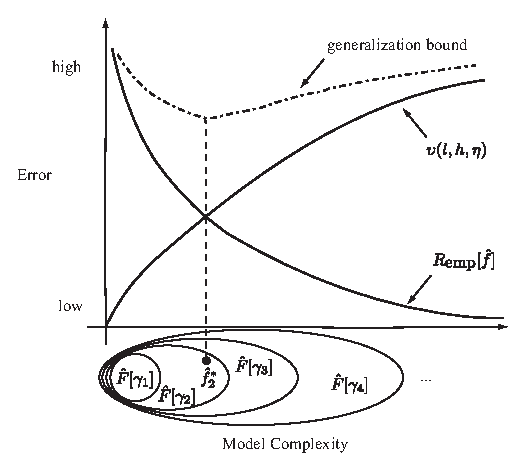
\includegraphics[height=45mm]{figures/fig10-07.eps}
\end{center}
Here we see that statistical learning theory and our intuitive notion of maximum margin 
classifier coincide.

In addition, statistical learning theory provides a nice mathematical 
framework for our intuitions.
\es
\end{document}
%%%%%%%%%%%%%%%%%%%%%%%%%%% end of template1.tex %%%%%%%%%%%%%%%%%%%%%%%%%%%%%%%%

